\chapter{Análise}	%The main chapter title
\chaptermark{Análise}	%Short version for page header. Comment if not needed
\label{Chapter4}

Neste capitulo será descrito o cenário requisitado, os requisitos funcionais, as restrições, atributos de qualidade e casos de uso. Também serão apresentados tabelas e diagramas que representam a arquitetura do protótipo.

\section{Descrição do cenário}

Um grupo de antigos alunos, alguns com experiência em Engenharia Informática, decidiram criar uma empresa dedicada à comercialização de sanduíches saudáveis numa loja física. Para isso é preciso criar uma solução informática que suporte as necessidades da mesma. É pretendido um sistema que tenha as capacidades necessárias para a gestão das várias dimensões da empresa. No desenvolvimento deste protótipo deve ser considerada uma arquitetura de microsserviços, bases de dados única para cada microsserviço e que esses mesmos devem ser chamados por meio de uma \textit{API Gateway}. A aplicação deve ser constituída por:
\begin{itemize}
\item Gestão de sanduíches
\item Gestão de ingredientes
\item Gestão de críticas
\item Gestão de lojas
\item Gestão de encomendas
\item Gestão de clientes
\end{itemize}

No sistema, cada sanduíche é identificada por uma designação, preço de venda e uma lista de ingredientes. Além disso, pode ter várias descrições, mas para idiomas autorizados, detetados pela própria aplicação. Qualquer sanduíche deve ser criada com o mínimo de 3 ingredientes, sendo obrigatório, conter um tipo da categoria de pão. Os ingredientes na lista devem ser verificados quanto a sua existência.

Um ingrediente possui uma designação e uma categoria, este é usado na formação da sanduíche.

Ao cliente é permitido criar uma crítica, onde é descrito a sua experiência após efetuar um pedido de sanduíche recorrendo a um comentário e uma escala de 0 a 5 estrelas. Deve ser feito uma filtragem inicial do conteúdo do comentário. Outros clientes podem indicar se gostaram ou não dessa crítica, mas também podem efetuar uma denúncia no caso de acharem que aquela crítica contém conteúdo ofensivas, entre outros. Posteriormente será revista por um administrador. Deve ser acompanhada da hora de criação.

Uma loja inclui uma designação da mesma, endereço e a pessoa responsável. Uma loja tem um horário de funcionamento que pode variar de dia para dia. A pessoa responsável possui um nome e um endereço eletrónico. O endereço da loja é constituído pela morada, número da porta, código postal, localidade e país.

Cada encomenda é composta pelo identificador do cliente que a efetuou, estado da encomenda, por uma lista de sanduíches e respetivas quantidades, bem como dia de entrega e a loja especifica de entrega, além disso, o protótipo deve informar o preço total da encomenda, deve-se ter em consideração que uma sanduíche não pode ser vendida abaixo de zero, apesar das promoções aplicadas.

Cada cliente inclui os seus detalhes pessoais, como nome, número de identificação fiscal, endereço, endereço eletrónico, dados de autenticação e idiomas que saiba falar. O endereço do cliente é constituído pela morada, número da porta, código postal, localidade e país.

As funcionalidades do administrador do sistema incluem criar, alterar e eliminar sanduíches, ingredientes e lojas, adicionar descrições, adicionar ingredientes às sanduíches e consultar informações dos clientes. A pessoa responsável pela loja tem como funcionalidades consultar informações dos clientes, verificar encomendas e alterar o estado das mesmas. Já as funcionalidades do cliente incluem visualizar informações sobre os seus dados de cliente, sanduíches, lojas, ingredientes e as suas encomendas.

O sistema deve responder em menos de 3 segundos a 10 utilizadores em simultâneo, conter um sistema de autenticação e autorização, ser modificável no que diz respeito a introdução de novas funcionalidades ou alteração de algumas já existentes, devem ser adotados testes nas várias dimensões, isto inclui as regras de negócio capturadas e o correto funcionamento da aplicação, ser implementado um sistema de mensagens via um \textit{message broker} e por último só é permitido o uso de tecnologias e ferramentas open source.

Dado que a empresa abrirá em breve, cerca de 3 meses, o \textit{software} deve estar disponível até a data de abertura.

\section{Modelo de Domínio}

Um modelo de domínio é usado para representar conceitos, objetos e relações com outros objetos que sejam importantes num determinado domínio de negócios. O modelo correspondente ao presente sistema pode ser visto na Figura \ref{fig:md}.

\begin{figure}[H]
    
\includegraphics[width=1.1\textwidth,left]{md.png}
    \caption{Modelo de Domínio}
    \label{fig:md}
\end{figure}

A Figura \ref{fig:md} apresenta os seguintes conceitos:
\begin{itemize}
    \item \textit{Customer}: Representa um utilizador
    \item \textit{PersonInCharge}: Representa uma pessoa responsável pela loja
    \item \textit{Person}: Representa uma pessoa em geral
    \item \textit{Address}: Representa um endereço
    \item \textit{AuthorizationData}: Representa dados de autorização
    \item \textit{Role}: Representa os cargos atribuídos a uma certa pessoa
    \item \textit{Sandwich}: Representa um sanduíche
    \item \textit{Description}: Representa uma descrição de uma sanduíche
    \item \textit{Ingredient}: Representa um ingrediente de uma sanduíche
    \item \textit{Category}: Representa uma categoria do ingrediente
    \item \textit{Review}: Representa uma avaliação de uma sanduíche
    \item \textit{Shop}: Representa uma loja
    \item \textit{OpeningHours}: Representa os horários de abertura de uma loja
    \item \textit{ClosingHours}: Representa os horários de encerramento de uma loja
    \item \textit{Order}: Representa um pedido
    \item \textit{OrderItem}: Representa um item do pedido
    \item \textit{ReviewAvaliation}: Representa a avaliação de uma revisão
    \item \textit{Language}: Representa um idioma
\end{itemize}

\section{Requisitos Funcionais}

Na tabela \ref{table:reqF} são apresentados os requisitos funcionais da aplicação, apresentam as caraterísticas e funcionalidades do sistema pretendido.
\begin{table}[H]
\caption{Requisitos Funcionais}
\label{table:reqF}
\begin{center}
\begin{tabular}{ |p{2cm}|p{4cm}|p{6cm}|  }
\hline
\multicolumn{3}{|c|}{Requisitos Funcionais} \\
\hline
\textbf{Referência} & \textbf{Requisito Funcional} & \textbf{Descrição} \\
\hline
RF1 & Gestão de sanduíches & O sistema disponibiliza  funcionalidades para a gestão de sanduíches \\
\hline
RF2 & Gestão de ingredientes & O sistema disponibiliza  funcionalidades para a gestão de ingredientes\\
\hline
RF3 & Gestão de críticas & O sistema disponibiliza  funcionalidades para a gestão de críticas\\
\hline
RF4 & Gestão de lojas & O sistema disponibiliza  funcionalidades para a gestão de lojas\\
\hline
RF5 & Gestão de encomendas & O sistema disponibiliza  funcionalidades para a gestão de encomendas\\
\hline
RF6 & Gestão de clientes & O sistema disponibiliza  funcionalidades para a gestão de clientes\\
\hline
\end{tabular} 
\end{center}
\end{table}

Os casos de uso são uma ferramenta valiosa na engenharia de \textit{software} para documentar e compreender os requisitos funcionais de um sistema. Por outro lado, os diagramas de caso de uso são as representações gráficas dos casos de uso, estes detalham as interações do sistema com todos os atores do mesmo. Podem ser definidas por meio de \ac{uml}, uma linguagem de modelagem que permite representar um sistema padronizada que pode ser utilizada na visualização, construção e na documentação de artefactos.

A seguir, serão apresentados os casos de uso por área, recorrendo a uma tabela que contém a referência do caso de uso e o diagrama que associa os mesmos aos respetivos atores, o agrupamento destes foi feito tendo em conta os vários elementos apresentados no cenário apresentado.

\subsection{Gestão de sanduíches}

Na Tabela \ref{table:sanduiche} são apresentados os casos de usos capturados para a gestão de sanduíches. Está acompanhada pela Figura \ref{fig:sanduiche}, diagrama de casos de usos para a administração de sanduíches.

\begin{table}[H]
\caption{Casos de usos para a gestão de sanduíches}
\label{table:sanduiche}
\begin{center}
\begin{tabular}{ |p{2cm}|p{10cm}|  }
\hline
\multicolumn{2}{|c|}{Casos de Uso} \\
\hline
\textbf{Referencia} & \textbf{Descrição} \\
\hline
UC05 & Criar uma sanduíche\\
\hline
UC06 & Obter uma sanduíche por ID\\
\hline
UC07 & Obter todas as sanduíches\\
\hline
UC09 & Adicionar descrição(ões) a uma sanduíche\\
\hline
UC10 & Obter todas as sanduíches que não possuam um ingrediente específico\\
\hline
UC30 & Alterar estado de um sanduíche\\
\hline
UC34 & Alterar os dados de uma sanduíche \\

\hline
\end{tabular} 
\end{center}
\end{table}

\begin{figure}[H]
    \centering
    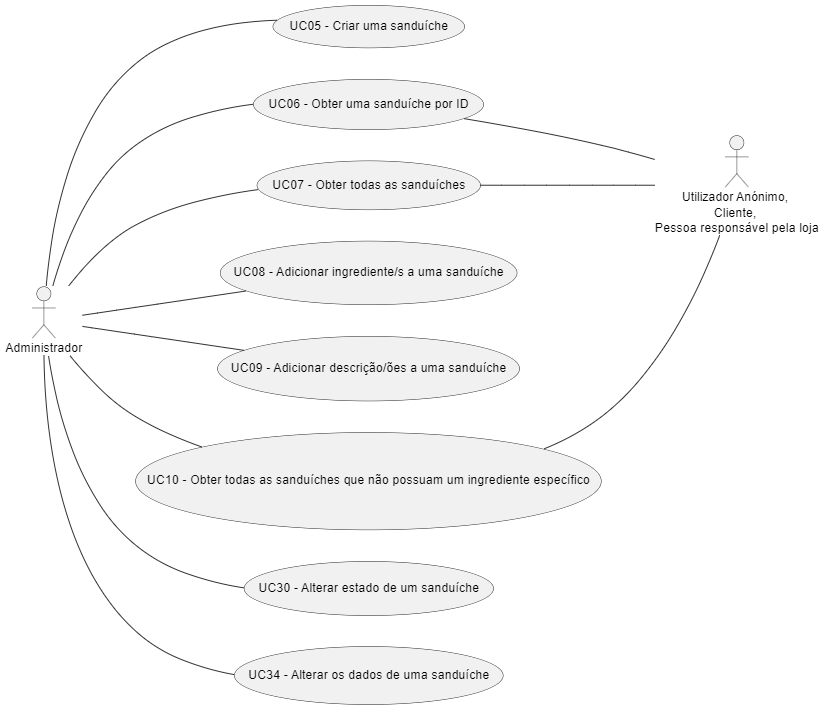
\includegraphics[scale=0.8]{sanduiche.png}
    \caption{Casos de usos para a gestão de sanduíches}
    \label{fig:sanduiche}
\end{figure}
	

\newpage

\subsection{Gestão de ingredientes}

Na Tabela \ref{table:ingredientes} são apresentados os casos de usos capturados para a gestão de ingredientes. Está acompanhada pela Figura \ref{fig:ingrediente}, diagrama de casos de usos para a administração de ingredientes.

\begin{table}[H]
\caption{Casos de usos para a gestão de ingredientes}
\label{table:ingredientes}
\begin{center}
\begin{tabular}{ |p{2cm}|p{10cm}|  }
\hline
\multicolumn{2}{|c|}{Casos de Uso} \\
\hline
\textbf{Referencia} & \textbf{Descrição} \\
\hline
UC01 & Criar um ingrediente\\
\hline
UC02 & Obter um ingrediente por ID\\
\hline
UC03 & Obter um ingrediente por designação\\
\hline
UC04 & Obter todos os ingredientes\\
\hline
UC29 & Alterar estado de um ingrediente\\
\hline
UC35 & Obter todos os ingredientes de uma certa categoria\\

\hline
\end{tabular} 
\end{center}
\end{table}

\begin{figure}[H]
    \centering
    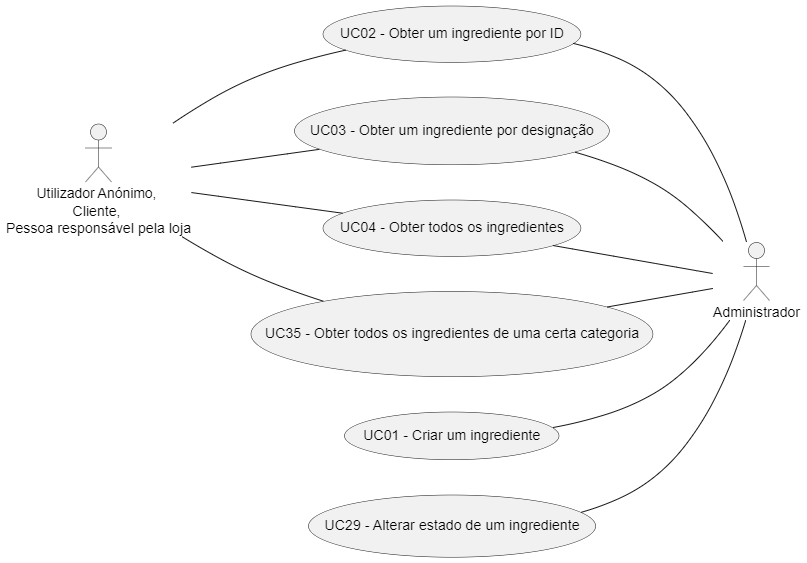
\includegraphics[scale=0.8]{ingrediente.png}
    \caption{Casos de usos para a gestão de ingredientes}
    \label{fig:ingrediente}
\end{figure}
\newpage

\subsection{Gestão de críticas}

Na Tabela \ref{table:criticas} são apresentados os casos de usos capturados para a gestão de críticas. Está acompanhada pela Figura \ref{fig:criticas}, diagrama de casos de usos para a administração de críticas.

\begin{table}[H]
\caption{Casos de usos para a gestão de críticas}
\label{table:criticas}
\begin{center}
\begin{tabular}{ |p{2cm}|p{10cm}|  }
\hline
\multicolumn{2}{|c|}{Casos de Uso} \\
\hline
\textbf{Referencia} & \textbf{Descrição} \\
\hline
UC19 & Adicionar crítica a uma sanduíche\\
\hline
UC20 & Votar numa crítica de uma sanduíche\\
\hline
UC21 & Listar todas as críticas de uma sanduíche\\
\hline
UC32 & Listar todas as críticas denunciadas\\
\hline
UC33 & Eliminar uma crítica denunciada por ID\\
\hline
UC36 & Denunciar uma crítica\\
\hline
UC43 & Editar uma crítica feita\\
\hline
UC44 & Listar todas as críticas feitas pelo cliente\\
\hline
UC45 & Eliminar critica feita pelo cliente\\

\hline
\end{tabular} 
\end{center}
\end{table}


\begin{figure}[H]
    \centering
    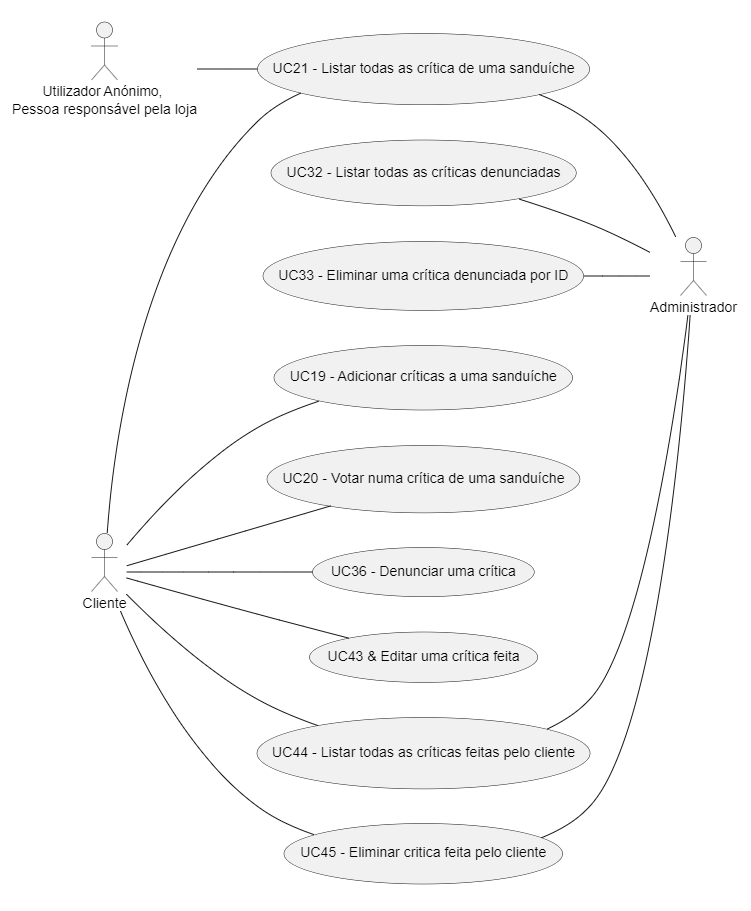
\includegraphics[scale=1]{critica.png}
    \caption{Casos de usos para a gestão de críticas}
    \label{fig:criticas}
\end{figure}
\newpage

\subsection{Gestão de lojas}

Na Tabela \ref{table:lojas} são apresentados os casos de usos capturados para a gestão de lojas. Está acompanhada pela Figura \ref{fig:loja}, diagrama de casos de usos para a administração de lojas.

\begin{table}[H]
\caption{Casos de usos para a gestão de lojas}
\label{table:lojas}
\begin{center}
\begin{tabular}{ |p{2cm}|p{10cm}|  }
\hline
\multicolumn{2}{|c|}{Casos de Uso} \\
\hline
\textbf{Referencia} & \textbf{Descrição} \\
\hline
UC22 & Criar loja\\
\hline
UC23 & Listar todas as lojas\\
\hline
UC24 & Listar loja por ID\\
\hline
UC25 & Listar loja por designação\\
\hline
UC26 & Listar loja por endereço\\
\hline
UC31 & Eliminar lojas\\
\hline
UC42 & Editar os dados de uma loja\\
\hline
\end{tabular} 
\end{center}
\end{table}

\begin{figure}[H]
    \centering
    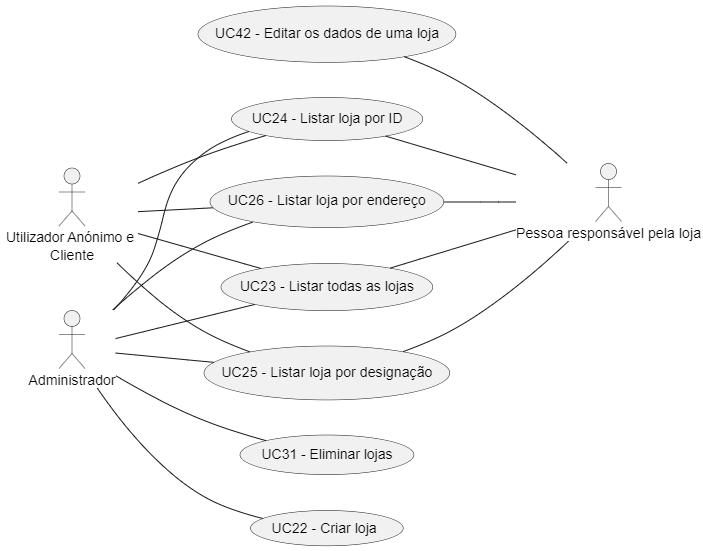
\includegraphics[scale=1]{loja.png}
    \caption{Casos de usos para a gestão de lojas}
    \label{fig:loja}
\end{figure}

\newpage
\subsection{Gestão de encomendas}

Na Tabela \ref{table:encomendas} são apresentados os casos de usos capturados para a gestão de encomendas. Está acompanhada pela Figura \ref{fig:encomendas}, diagrama de casos de usos para a administração de encomendas.

\begin{table}[H]
\caption{Casos de usos para a gestão de encomendas}
\label{table:encomendas}
\begin{center}
\begin{tabular}{ |p{2cm}|p{10cm}|  }
\hline
\multicolumn{2}{|c|}{Casos de Uso} \\
\hline
\textbf{Referencia} & \textbf{Descrição} \\
\hline
UC27 & Criar uma encomenda\\
\hline
UC28 & Listar encomendas de uma loja\\
\hline
UC37 & Alterar a estado da encomenda\\
\hline
UC39 & Listar as encomendas do cliente\\
\hline
\end{tabular} 
\end{center}
\end{table}

\begin{figure}[H]
    \centering
    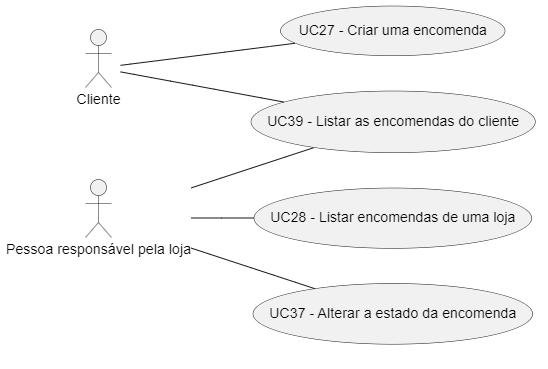
\includegraphics[scale=0.8]{encomenda.png}
    \caption{Casos de usos para a gestão de encomendas}
    \label{fig:encomendas}
\end{figure}

\newpage

\subsection{Gestão de clientes}

Na Tabela \ref{table:clientes} são apresentados os casos de usos capturados para a gestão de clientes. Está acompanhada pela Figura \ref{fig:clientes}, diagrama de casos de usos para a administração de clientes.

\begin{table}[H]
\caption{Casos de usos para a gestão de clientes}
\label{table:clientes}
\begin{center}
\begin{tabular}{ |p{2cm}|p{10cm}|  }
\hline
\multicolumn{2}{|c|}{Casos de Uso} \\
\hline
\textbf{Referencia} & \textbf{Descrição} \\
\hline
UC11 & Adicionar cliente\\
\hline
UC12 & Obter cliente por ID\\
\hline
UC13 & Obter cliente por e-mail\\
\hline
UC14 & Obter cliente por número de identificação fiscal\\
\hline
UC15 & Obter dados de autenticação do cliente\\
\hline
UC16 & Obter todos os clientes\\
\hline
UC17 & Adicionar permissões a um cliente\\
\hline
UC18 & Fazer \textit{login}\\
\hline
UC40 & Alterar os dados do cliente\\
\hline
UC41 & Visualizar os dados do cliente\\


\hline
\end{tabular} 
\end{center}
\end{table}

\begin{figure}[H]
    \centering
    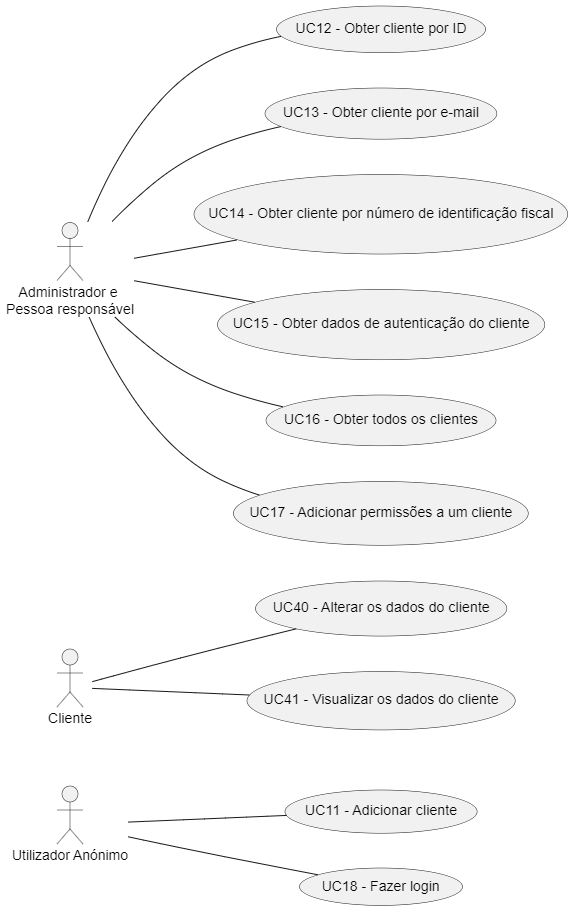
\includegraphics[scale=0.9]{cliente.png}
    \caption{Casos de usos para a gestão de clientes}
    \label{fig:clientes}
\end{figure}

\newpage

\section{Restrições}

Na tabela \ref{table:restricoes} são apresentadas as restrições que afetam o desenvolvimento do projeto de \textit{software}.

\begin{table}[H]
\caption{Restrições}
\label{table:restricoes}
\begin{center}
\begin{tabular}{ |p{3cm}|p{3cm}|p{6cm}|  }
\hline
\multicolumn{3}{|c|}{Restrições} \\
\hline
\textbf{Referência} & \textbf{Restrição} & \textbf{Descrição} \\
\hline
R1 & Linguagem & O protótipo deve ser escrito recorrendo a Ballerina\\
\hline
R2 & Arquitetura de microsserviços &  A solução deve utilizar a arquitetura de microsserviços\\
\hline
R3 & Aplicações e ferramentas open source & Só são permitidas aplicações e ferramentas open source no desenvolvimento do sistema\\
\hline
R4 & Tempo & A aplicação deve estar concluída em três meses\\
\hline
\end{tabular} 
\end{center}
\end{table}


\section{Atributos de Qualidade}

Na Tabela \ref{table:qualidades} são apresentadas os atributos de qualidade que o sistema deve apresentar recorrendo à norma ISO 25010, que define a qualidade do \textit{software} como um conjunto de características que o mesmo deve possuir para atender às necessidades pretendidas. Esta norma é representada por 8 categorias:
\begin{itemize}
    \item Adequação funcional \cite{iso25010cat}
    \item Eficiência de desempenho \cite{iso25010cat}
    \item Compatibilidade \cite{iso25010cat}
    \item Usabilidade \cite{iso25010cat}
    \item Confiabilidade \cite{iso25010cat}
    \item Segurança \cite{iso25010cat}
    \item Manutenibilidade \cite{iso25010cat}
    \item Portabilidade \cite{iso25010cat}
\end{itemize}

\begin{table}[H]
\caption{Atributos de Qualidade}
\label{table:qualidades}
\begin{center}
\begin{tabular}{ |p{3cm}|p{3cm}|p{6cm}|  }
\hline
\multicolumn{3}{|c|}{Atributos de Qualidade} \\
\hline
\textbf{Referência} & \textbf{Atributo} & \textbf{Descrição} \\
\hline
Q1 & Segurança & Mecanismos de autenticação e autorização devem ser implementados\\
\hline
Q2 & Desempenho & A aplicação deve responder as pedidos realizados por 10 utilizadores em simultâneo em menos de 3 segundos\\
\hline
Q3 & Manutenibilidade & Pretende-se que a aplicação possa evoluir, pelo que, deverão ser aplicados padrões de \textit{design} apropriados\\
\hline
\end{tabular} 
\end{center}
\end{table}

Adicionalmente, relativamente ao atributo de qualidade com referência Q1, deve ser mencionado que deverão ser seguidos as dez principais práticas para o desenvolvimento de código seguro. As dez principais práticas são constituídas por:
\begin{itemize}
    \item Validação de todas as entradas de fontes de dados não seguras \cite{top10}
    \item Ter atenção aos avisos do compilador e recorrer a ferramentas de análise estática e dinâmica para identificar e eliminar falhas de segurança \cite{top10}
    \item Criar uma arquitetura de software e conceber o seu software para implementar e aplicar políticas de segurança. \cite{top10}
    \item Desenhar um sistema o mais simples e pequeno possível \cite{top10}
    \item O acesso deve ser baseado em permissões em vez de exclusões \cite{top10}
    \item Cada processo deve ter o menor conjunto de privilégios necessários para concluir o trabalho \cite{top10}
    \item Os dados enviados para um sistema complexos devem passar por um processo de limpeza \cite{top10}
    \item Deve ser feito uma gestão de risco com múltiplas estratégias defensivas para prevenir falhas de segurança e limitar as consequências de um possível \textit{exploit} \cite{top10}
    \item Deve ser incorporado testes de qualidade do código-fonte, testes de penetração e testes de \textit{fuzz} \cite{top10}
    \item Desenvolver um padrão de codificação seguro para a linguagem e plataforma de desenvolvimento utilizada \cite{top10}
\end{itemize}








